\documentclass[preprint, 3p,
authoryear]{elsarticle} %review=doublespace preprint=single 5p=2 column
%%% Begin My package additions %%%%%%%%%%%%%%%%%%%

\usepackage[hyphens]{url}

  \journal{Ursus} % Sets Journal name

\usepackage{graphicx}
%%%%%%%%%%%%%%%% end my additions to header

\usepackage[T1]{fontenc}
\usepackage{lmodern}
\usepackage{amssymb,amsmath}
% TODO: Currently lineno needs to be loaded after amsmath because of conflict
% https://github.com/latex-lineno/lineno/issues/5
\usepackage{lineno} % add
\usepackage{ifxetex,ifluatex}
\usepackage{fixltx2e} % provides \textsubscript
% use upquote if available, for straight quotes in verbatim environments
\IfFileExists{upquote.sty}{\usepackage{upquote}}{}
\ifnum 0\ifxetex 1\fi\ifluatex 1\fi=0 % if pdftex
  \usepackage[utf8]{inputenc}
\else % if luatex or xelatex
  \usepackage{fontspec}
  \ifxetex
    \usepackage{xltxtra,xunicode}
  \fi
  \defaultfontfeatures{Mapping=tex-text,Scale=MatchLowercase}
  \newcommand{\euro}{€}
\fi
% use microtype if available
\IfFileExists{microtype.sty}{\usepackage{microtype}}{}
\usepackage[]{natbib}
\bibliographystyle{plainnat}

\usepackage{graphicx}
\ifxetex
  \usepackage[setpagesize=false, % page size defined by xetex
              unicode=false, % unicode breaks when used with xetex
              xetex]{hyperref}
\else
  \usepackage[unicode=true]{hyperref}
\fi
\hypersetup{breaklinks=true,
            bookmarks=true,
            pdfauthor={},
            pdftitle={Loss of habitat and connectivity for the Spectacled Bear Tremarctos ornatus in Colombia, and evaluation of the role of Protected Areas and communal territories in its conservation},
            colorlinks=false,
            urlcolor=blue,
            linkcolor=magenta,
            pdfborder={0 0 0}}

\setcounter{secnumdepth}{5}
% Pandoc toggle for numbering sections (defaults to be off)


% tightlist command for lists without linebreak
\providecommand{\tightlist}{%
  \setlength{\itemsep}{0pt}\setlength{\parskip}{0pt}}

% From pandoc table feature
\usepackage{longtable,booktabs,array}
\usepackage{calc} % for calculating minipage widths
% Correct order of tables after \paragraph or \subparagraph
\usepackage{etoolbox}
\makeatletter
\patchcmd\longtable{\par}{\if@noskipsec\mbox{}\fi\par}{}{}
\makeatother
% Allow footnotes in longtable head/foot
\IfFileExists{footnotehyper.sty}{\usepackage{footnotehyper}}{\usepackage{footnote}}
\makesavenoteenv{longtable}






\begin{document}


\begin{frontmatter}

  \title{Loss of habitat and connectivity for the Spectacled Bear
\emph{Tremarctos ornatus} in Colombia, and evaluation of the role of
Protected Areas and communal territories in its conservation}
    \author[UdeM]{Cristian A. Cruz-Rodríguez%
  \corref{cor1}%
  \fnref{1}}
   \ead{cruzrodriguezcristian@gmail.com} 
    \author[IAvH]{Sergio Rojas%
  %
  \fnref{2}}
   \ead{srojas@humboldt.org.co} 
    \author[IAvH]{Sergio Rojas%
  %
  \fnref{2}}
   \ead{srojas@humboldt.org.co} 
    \author[ProCAT]{Maria Camila Machado-Aguilera%
  %
  \fnref{2}}
   \ead{camimachado12@hotmail.com} 
    \author[]{Diego Andrés Zárrate-Charry%
  %
  \fnref{2}}
   \ead{godiezcharry@gmail.com} 
      \affiliation[UdeM]{
    organization={Université de
Montréal},city={Montréal},state={Quebec},country={Canada},}
    \affiliation[IAvH]{
    organization={Instituto de Investigación de Recursos Biológicos
Alexander von Humboldt},city={Bogotá D.C.},country={Colombia},}
    \affiliation[ProCAT]{
    organization={Proyecto de Conservación de Aguas y Tierras - ProCAT
Colombia},city={Bogotá D. C.},country={Colombia},}
    \cortext[cor1]{Corresponding author}
    \fntext[1]{This is the first author footnote.}
    \fntext[2]{Another author footnote.}
  
  \begin{abstract}
  The spectacled bear (Tremarctos ornatus) is an endemic species that
  was associated with humid forest areas of the Neotropical Andes. It
  plays an important role in seed dispersal and succession processes. It
  is currently categorized as vulnerable due to the loss and
  fragmentation of its habitat, and retaliatory hunting. In the present
  study, the historical distribution of the species was identified for
  the changes in coverage in recent years established the bear-community
  conflict zones in the country. The results will serve as inputs to
  prioritize conservation areas and generate strategies that minimize
  conflict with communities.
  \end{abstract}
    \begin{keyword}
    Ecological changes \sep Fragmentation \sep Multitemporal
Analysis \sep Neural analalisiis \sep 
    threatened species
  \end{keyword}
  
 \end{frontmatter}

\hypertarget{introduction}{%
\section{Introduction}\label{introduction}}

The spectacled bear (\emph{Tremarctos ornatus}) was found in southern
California and Central America, but after the Pleistocene, it was
reduced to South America
\citep{Paisley2006Activity, Vela-Vargas2021Tremarctos} It is currently
the only species of the family Ursidae in the Neotropics and its
historical distribution included from the department of Mérida in
Venezuela to southern Bolivia, in the department of Tarija, and possibly
in some regions of northern Argentina
\citep{Garcia-Rangel2012Andean, Goldstein2006Andean}.

Research on the spectacled bear has been conducted in Colombia since
1985. However, to date, knowledge about ecological aspects and the
status of their populations is still approximate
\citep{Kattan2004Range}. This species is threatened by the high rate of
habitat transformation, which in the 1980s was 60,000 - and has probably
increased due to the presence of illicit crops and human population
growth in recent years \citep{Rodriguez2003Ecoregional}. Additionally,
there has been an increase in bear-community conflict due to attacks on
livestock and crop losses associated with the presence of bears, which
may be due to the decrease in food supply in their natural habitat and
the presence of livestock in and around their areas of use
\citep{Kattan2004Range, Sanchez-Mercado2008Factors}.

Regarding conservation efforts, the formation of the Frontine Bear
Specialist Group (GEOF) in 1983 gave rise to the Action Plan for the
Conservation of the World's Bears by the IUCN. Based on this initiative,
in Colombia, the Ministry of the Environment, together with several NGOs
and regional autonomous corporations, participated in the formulation of
the National Conservation Program for Tremarctos ornatus in 2001 and the
Ecoregional Strategy for the Conservation of the Andean Bear in the
Northern Andes in 2003. Likewise, work is currently being done on the
Chingaza-Sumapaz-Guerrero Conservation Corridor initiative, which
includes a large part of the species distribution in the departments of
Cundinamarca and Meta \citep{Quintero2023Andean}. This corridor emerged
as a strategy to achieve regional natural connectivity and to protect
areas of water importance \citep{Quintero2023Andean} and in this sense,
the inclusion of the bear as an umbrella species could help the
conservation of the ecosystems of high mountains and water resources
\citep{Kattan2004Range}.

The main objective of this article was to evaluate the trend of change
in habitat availability and elements of potential connectivity for the
Spectacled Bear in Colombia in the last two decades and the role that
PAs have played in its conservation. Likewise, the priority conservation
units of the species related to its viability will be evaluated at the
national level due to its potential to maintain a population, and key
landscapes to ensure connectivity.@Kattan2004Range

\hypertarget{materials-and-methods}{%
\section{Materials and Methods}\label{materials-and-methods}}

\hypertarget{species-distribution-model}{%
\subsection{Species Distribution
Model}\label{species-distribution-model}}

The Potential Distribution Model available on the BioModelos Web portal
(\emph{www.biomodelos.org.co}) was used. BioModelos is a collaborative
tool that created Species Distribution Models using mathematical methods
and expert opinions \citep{Velasquez-Tibata2019Biomodelos} (Fig. 1).
Likewise, information was collected in the communities surrounding the
study area seeking to identify the sectors in which the spectacled bear
has had direct or indirect contact with a man. The places of
bear-community conflict will be georeferenced and located on the
probability of presence maps, to infer how the conflicts are related to
the probability of presence of the species.

\hypertarget{identification-of-habitat-coverage}{%
\subsection{Identification of habitat
coverage}\label{identification-of-habitat-coverage}}

A search was carried out in the literature of the covers that have been
reported as bear habitat. The search was carried out mainly on the Web
of Science and in Google Scholar, using the following keywords;
Tremarctos ornatus, Andean bear, spectacled bear, Andean bear,
spectacled bear, and habitat. Subsequently, the coverages found were
validated based on coverages reported by experts, the IUCN,
\citet{Nowak1999Walker}, \citet{Hunt1998Ursidaea}, and
\citet{Garshelis2009Family}. The covers with at least one support from
the sources mentioned above were taken as the covers with habitat for
the species, thus selecting the covers of open forest, dense forest,
riparian forest, grasslands, fragmented forest, secondary vegetation,
and shrubs.

\hypertarget{identification-of-habitat-patches}{%
\subsection{Identification of habitat
patches}\label{identification-of-habitat-patches}}

To identify remaining habitat patches for the species in different
periods, the national coverage layers available for the years 2002,
2012, and 2018 were taken. Subsequently, only the previously defined
coverages were selected and the layer continued to be dissolved. to have
a simpler one. With this, the cover layers were cut, for the different
years, with the distribution model of the species, to obtain an
approximation of the habitats occupied by the species. Finally, the
areas were calculated, and only patches with sizes equal to or greater
than 20 Km were selected.

\hypertarget{results-and-discussion}{%
\section{Results and discussion}\label{results-and-discussion}}

It exists and is around in records reported in the last year to the
species. Principally in the last 25 years (fig 2). This situation is
probably because the use of the new technologies is more shipper than in
another year and increased the use of tools to report the presence of
the species. From the results obtained, the records of the species match
with the ecosystems that have been reported in the bibliography, since
the species is found in different ecosystems, among which dry areas
stand out (in coastal sectors of Peru), areas of desert, and thorny
chaparral to Páramos and cloud forests along the Andes mountain range
\citet{Kattan2004Range}, \citet{Garcia-Rangel2012Andean})

About the places in which the presence of the species was reported, in
data portals Colombia was the country with the most records for this
species (tale 1) To Colombia the was observed that these largely
coincided with those present for Colombia, since in addition to
inhabiting the three mountain ranges that cross the country, there are
records that locate the species in the Sierra Nevada de Santa Marta, in
the Serranía de Perijá \citet{Solari2013Riqueza} , in the Serranía de
Baudó and the Macarena \citep{Vela-Vargas2021Tremarctos}

As for what was recorded by the model, the values obtained coincide with
those recorded in other studies for the species, being evident in the
important statistical robustness achieved with the study, despite not
having had records for the species in its entire area
\citep{MezaMori2020Predictive}.

\begin{figure}

{\centering 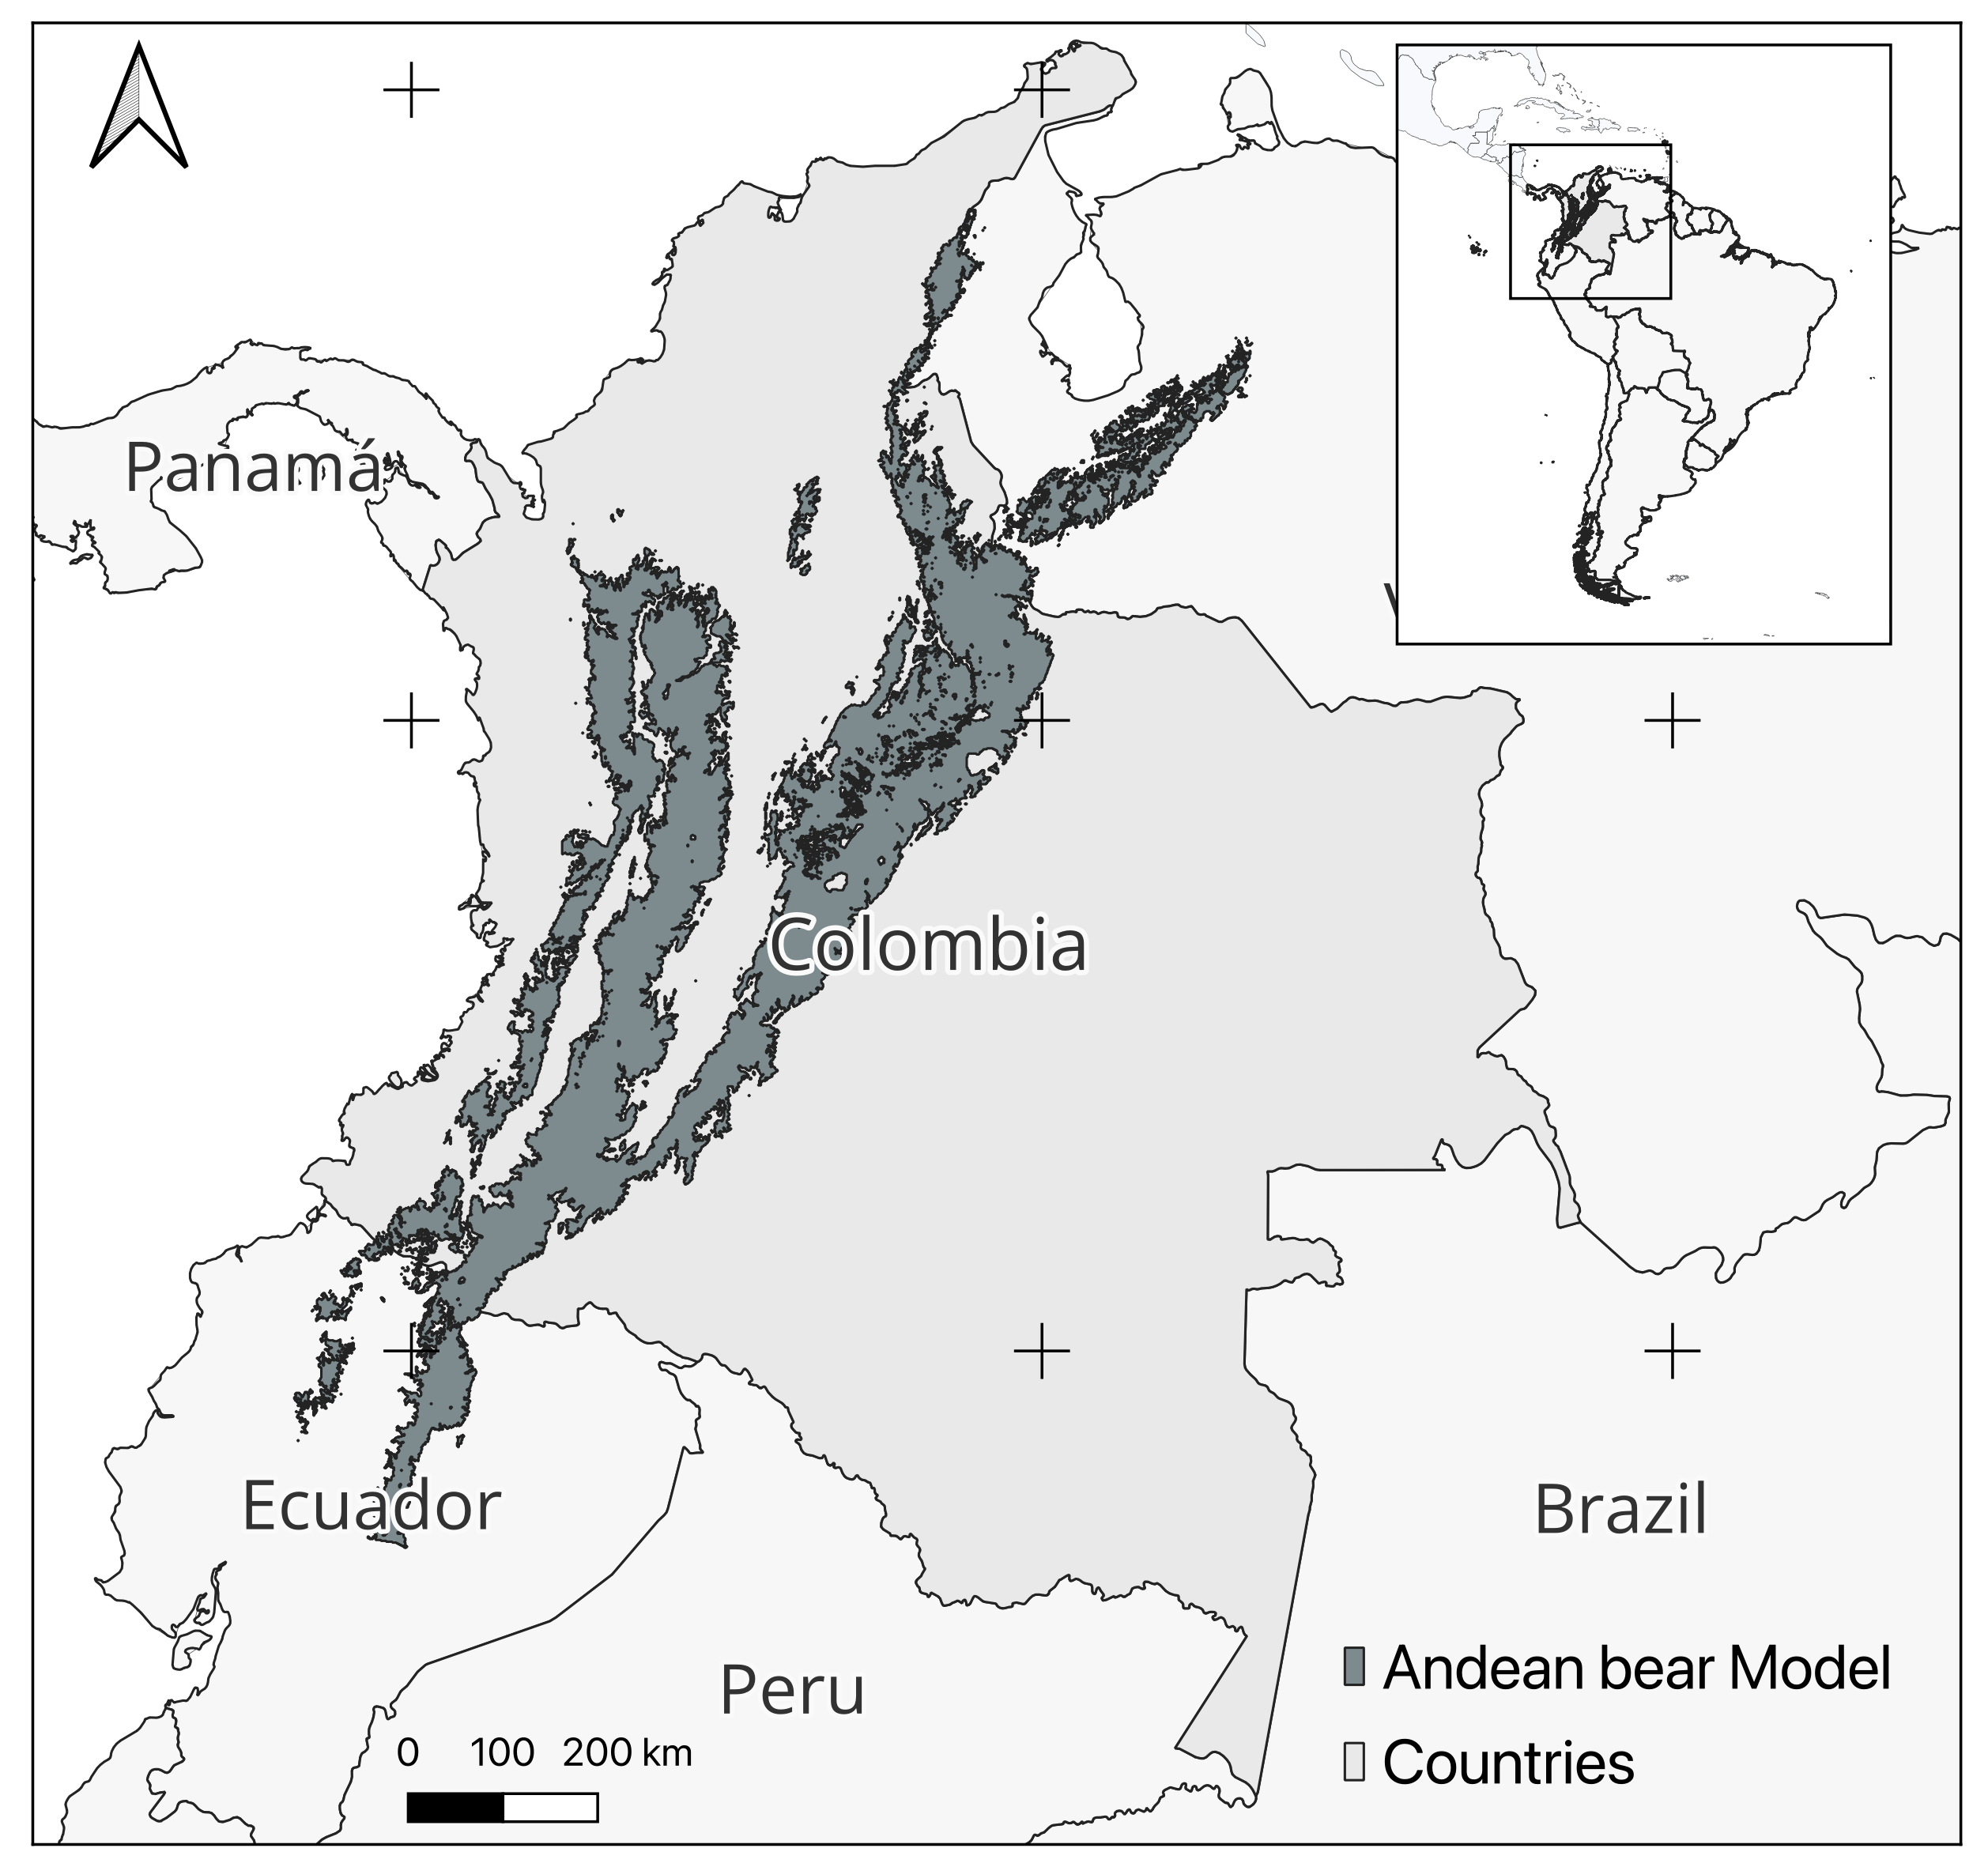
\includegraphics[width=1\linewidth]{../figures/Figure1} 

}

\caption{Potentianl distribution to the Andean Bear in the North of the Andes}\label{fig:unnamed-chunk-1}
\end{figure}

\begin{figure}
\centering
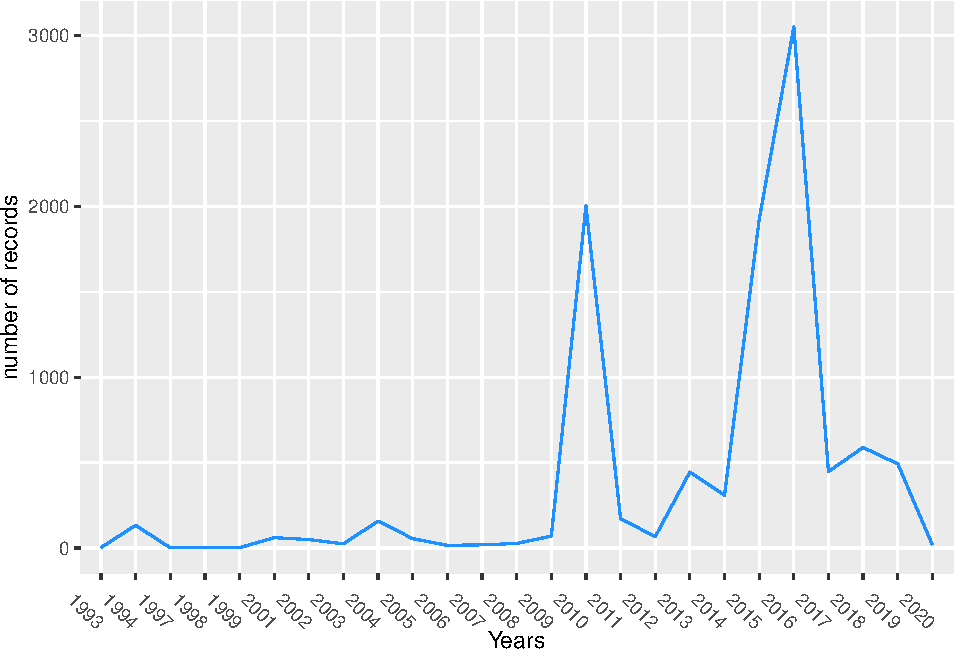
\includegraphics{manuscript_files/figure-latex/theme_ggplot2-1.pdf}
\caption{Records to the Andean bear in the las 25 years}
\end{figure}

\begin{longtable}[]{@{}lr@{}}
\caption{\label{tab1}Records by countriess}\tabularnewline
\toprule\noalign{}
Countries & Frecuency \\
\midrule\noalign{}
\endfirsthead
\toprule\noalign{}
Countries & Frecuency \\
\midrule\noalign{}
\endhead
\bottomrule\noalign{}
\endlastfoot
Colombia & 10339 \\
Ecuador & 58 \\
Panamá & 1 \\
Perú & 944 \\
Venezuela & 2 \\
\end{longtable}

\bibliography{mybibfile.bib}


\end{document}
